\documentclass[11pt]{scrreprt}
\usepackage[T1]{fontenc}
\usepackage[utf8]{inputenc}
\usepackage[french]{babel}
\usepackage[scale=0.775]{geometry}
\usepackage{lmodern}
\usepackage[ilines]{scrpage2}
\usepackage[pdftex, bookmarks=true, hidelinks]{hyperref}
\usepackage{graphicx}
\usepackage{tocbibind}
\usepackage{chngcntr}
\usepackage{tabularx}
\usepackage{float}
\usepackage{scrhack}
\usepackage{ulem}
\usepackage{enumitem}
\usepackage{subfigure}

\counterwithout{figure}{chapter}
\counterwithout{table}{chapter}
\pagestyle{scrheadings}

% clear head and foot
\clearscrheadings
\clearscrplain
\clearscrheadfoot

\cefoot[\textsc{Nathan Raspe \& Matteo Taroli}]{\textsc{Nathan Raspe \& Matteo Taroli}}
\cofoot[\textsc{Nathan Raspe \& Matteo Taroli}]{\textsc{Nathan Raspe \& Matteo Taroli}}
\lefoot[]{}
\lofoot[]{}
\refoot[\thepage]{\thepage}
\rofoot[\thepage]{\thepage}

\begin{document}

    \renewcommand{\labelitemi}{$\bullet$}
    \renewcommand{\labelitemii}{$\circ$}
    %%%%%% TITLE PAGE %%%%%%%%%%%%%%%%%%%
    \begin{titlepage}
        \begin{center}
            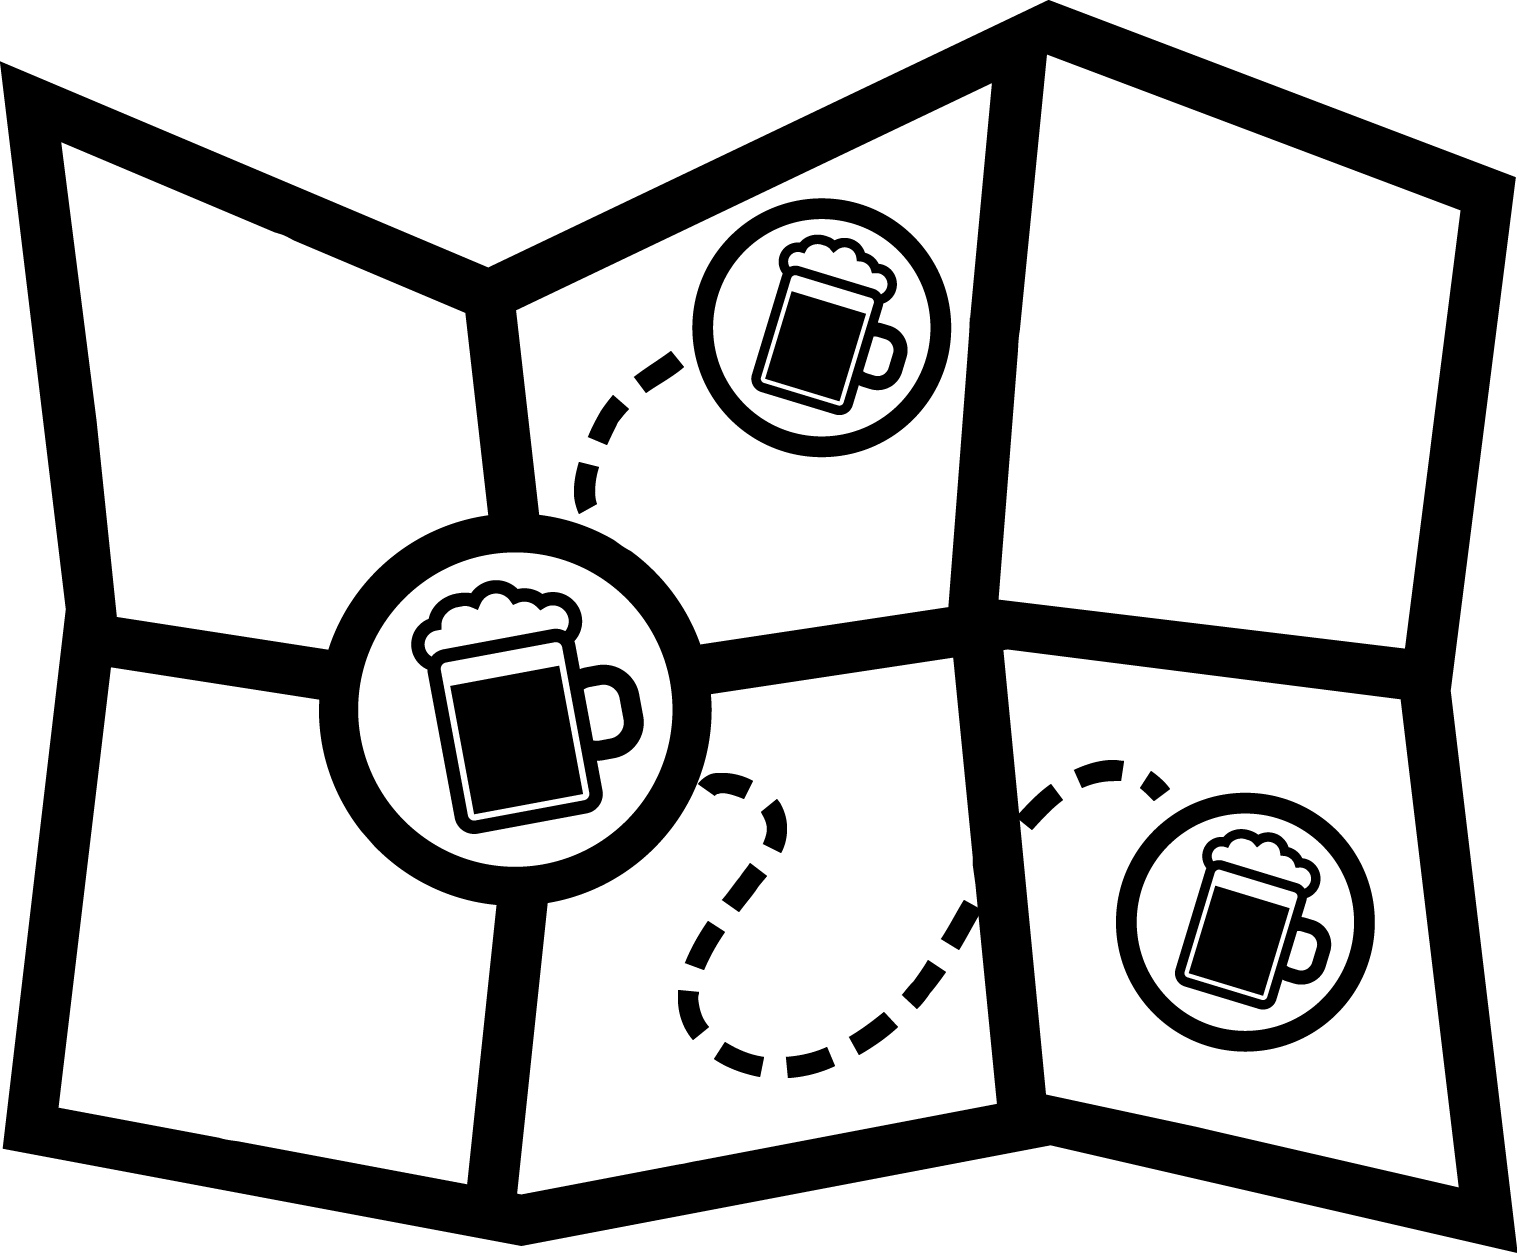
\includegraphics[width=10cm]{images/logo.png}
            ~\\[1.5cm]

            % Title
            \rule{\textwidth}{1pt} \\[0.4cm]
            \Huge{\textsc{\textbf{History Pub}}}\\ \Large{\textit{Découvrez Soignies en boisson}\\[0.4cm]}

            \rule{\textwidth}{1pt} \\[1.5cm]

            \textsc{\Large Projet de Développement d'Application Mobile}\\[0.5cm]

            % Authors
            Nathan Raspe \& Matteo Taroli

            \vfill

            {\large 27 Novembre 2015}
            \vfill
        \end{center}
    \end{titlepage}

    % Table of contents
    \pagenumbering{roman}
    \tableofcontents
    % List of figures
    \renewcommand\listfigurename{Table des illustrations}
    \listoffigures
    \pagebreak
    \pagenumbering{arabic}

    %%%%%%%% BEGIN CONTENT %%%%%%%%%%%%
    \chapter{Introduction}
    Dans le cadre du cours de Dévelopement d'Application Mobile, nous avons dû développer une application reprenant le concept du jeu de piste. Cette application, nommée \textsc{History Pub} vous propose de découvrir la ville de Soignies en passant par les différents bars qu'offre celle-ci.\\

    Sur le chemin entre ces différents établissements, vous aurez l'occasion d'en apprendre plus sur l'histoire et le folklore de la ville. Durant les différents arrêts, vous aurez bien entendu l'occasion de profiter des bars et des diverses boissons proposées avant de reprendre le chemin vers d'autres découvertes!\\

    Attention tout de même, l'alcool est à consommer avec modération, sous peine de ne plus pouvoir répondre aux questions données!\\

    \chapter{Mode d'emploi}
    L'utilisation de \textsc{History Pub} est très facile. Une fois l'application lancée, vous recevez les indications vous permettant de trouver la zone de la première étape du jeu.

    % Afficher une screenshot de EtapeActivité demandant de se déplacer dans la zone

    Une fois dans la zone, et après avoir lu une courte description de l'endroit et où de son histoire, vous vous retrouverez devant une épreuve qui peut prendre différentes formes. Ces épreuves sont décrites ci-dessous.

    \section{Caractéristiques communes aux épreuves}
    Lors des épreuves de question à choix multiples ou de question ouvertes, votre réponse doit être vérifiée. Cette vérification n'est faite qu'une fois la réponse validée par l'utilisateur, c'est à dire une fois que le bouton OK est pressé. Cette vérification peut mener à trois différents toast possibles :
    \begin{description}[style=nextline]
        \item[Pas de réponse donnée]Un toast invite l'utilisateur à répondre à la question.
        \item[Réponse correcte]Une fenêtre popup apparait pour féliciter l'utilisateur et afficher le nombre de points gagnés.
        \item[Réponse incorrecte]La fenêtre popup se désole de la mauvaise réponse et donne la réponse correcte, permettant à l'utilisateur d'apprendre de ses erreurs.
    \end{description}
    Dans les deux cas où une réponse est donnée, la fenêtre popup donne de plus ample informations par rapport à la réponse à la question, comme vous pouvez le voir sur la capture d'écran suivante. Cette fenêtre permet aussi de partager l'avancement dans le jeu.

    De plus, 2 autres boutons sont également présents. Ceux-ci sont communs à toutes les épreuves, réalisent les mêmes actions mais de manières différentes en fonction du type d'épreuve. (Voir sections 2.2 à 2.5)
    \begin{description}[style=nextline]
        \item[Bouton de triche]Ce bouton sert à obtenir la réponse de l'épreuve. Aucun point ne sera accordé à l'utilisateur si ce bouton est pressé. L'aide et la triche ne seront plus disponibles.
        \item[Bouton d'aide]Ce bouton sert à obtenir un indice. La moitié des points sera accordé à l'utilisateur si ce bouton est pressé. L'aide n'est plus disponible.
    \end{description}

    \section{Epreuve Question à Choix Multiple}
    \begin{figure}[H]
        \centering
        \mbox{\subfigure{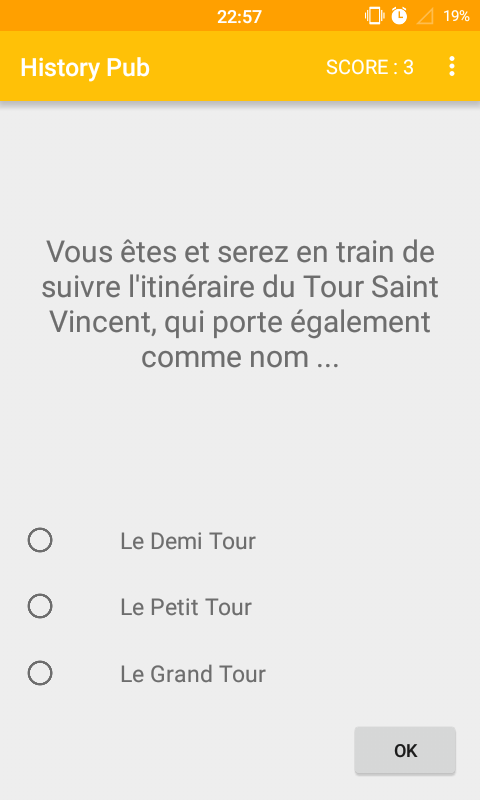
\includegraphics[scale=.25]{images/qcm1.png}}\quad\quad\quad
        \subfigure{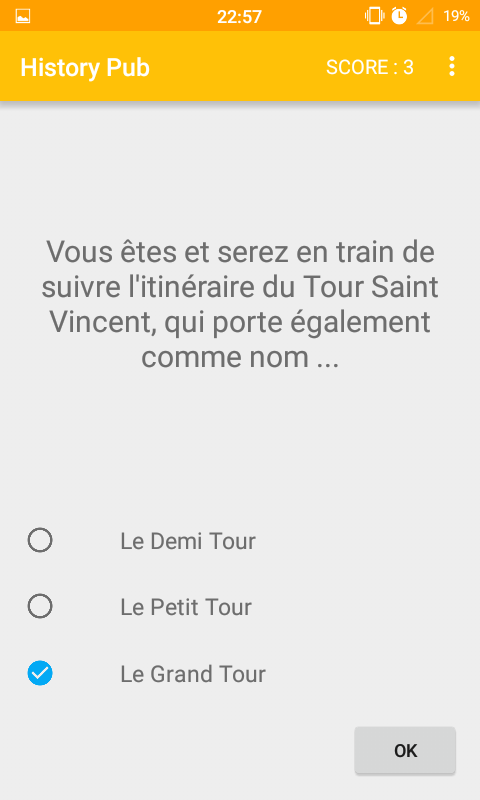
\includegraphics[scale=.25]{images/qcm2.png}}}
        \caption{Exemple de question à choix multiple, avant et après avoir sélectionné une réponse}
    \end{figure}

    Pour répondre à une question à choix multiples, il vous suffit de cliquer sur la réponse que vous pensez correcte. Vous pouvez cliquer n'importe où sur la ligne de ce choix, que ce soit sur la checkbox ou sur le texte de la réponse proposée.\\

    Un symbole $\surd$ s'affiche dans la checkbox de la réponse sélectionnée. Si celle ci vous convient, vous pouvez confirmer votre choix grâce au bouton OK. Sinon, vous êtes libre de changer ce choix autant de fois que vous le désirez.\\

    Pour ce type d'épreuve:
    \begin{description}[style=nextline]
        \item[Bouton de triche]Il retire toutes les réponses incorrectes et coche automatiquement la bonne réponse. Il faut ensuite appuyer sur le bouton OK.
        \item[Bouton d'aide]Il enlève aléatoirement une mauvaise réponse.
    \end{description}

    \section{Epreuve de texte à trous}
    \begin{figure}[H]
        \centering
        \mbox{\subfigure{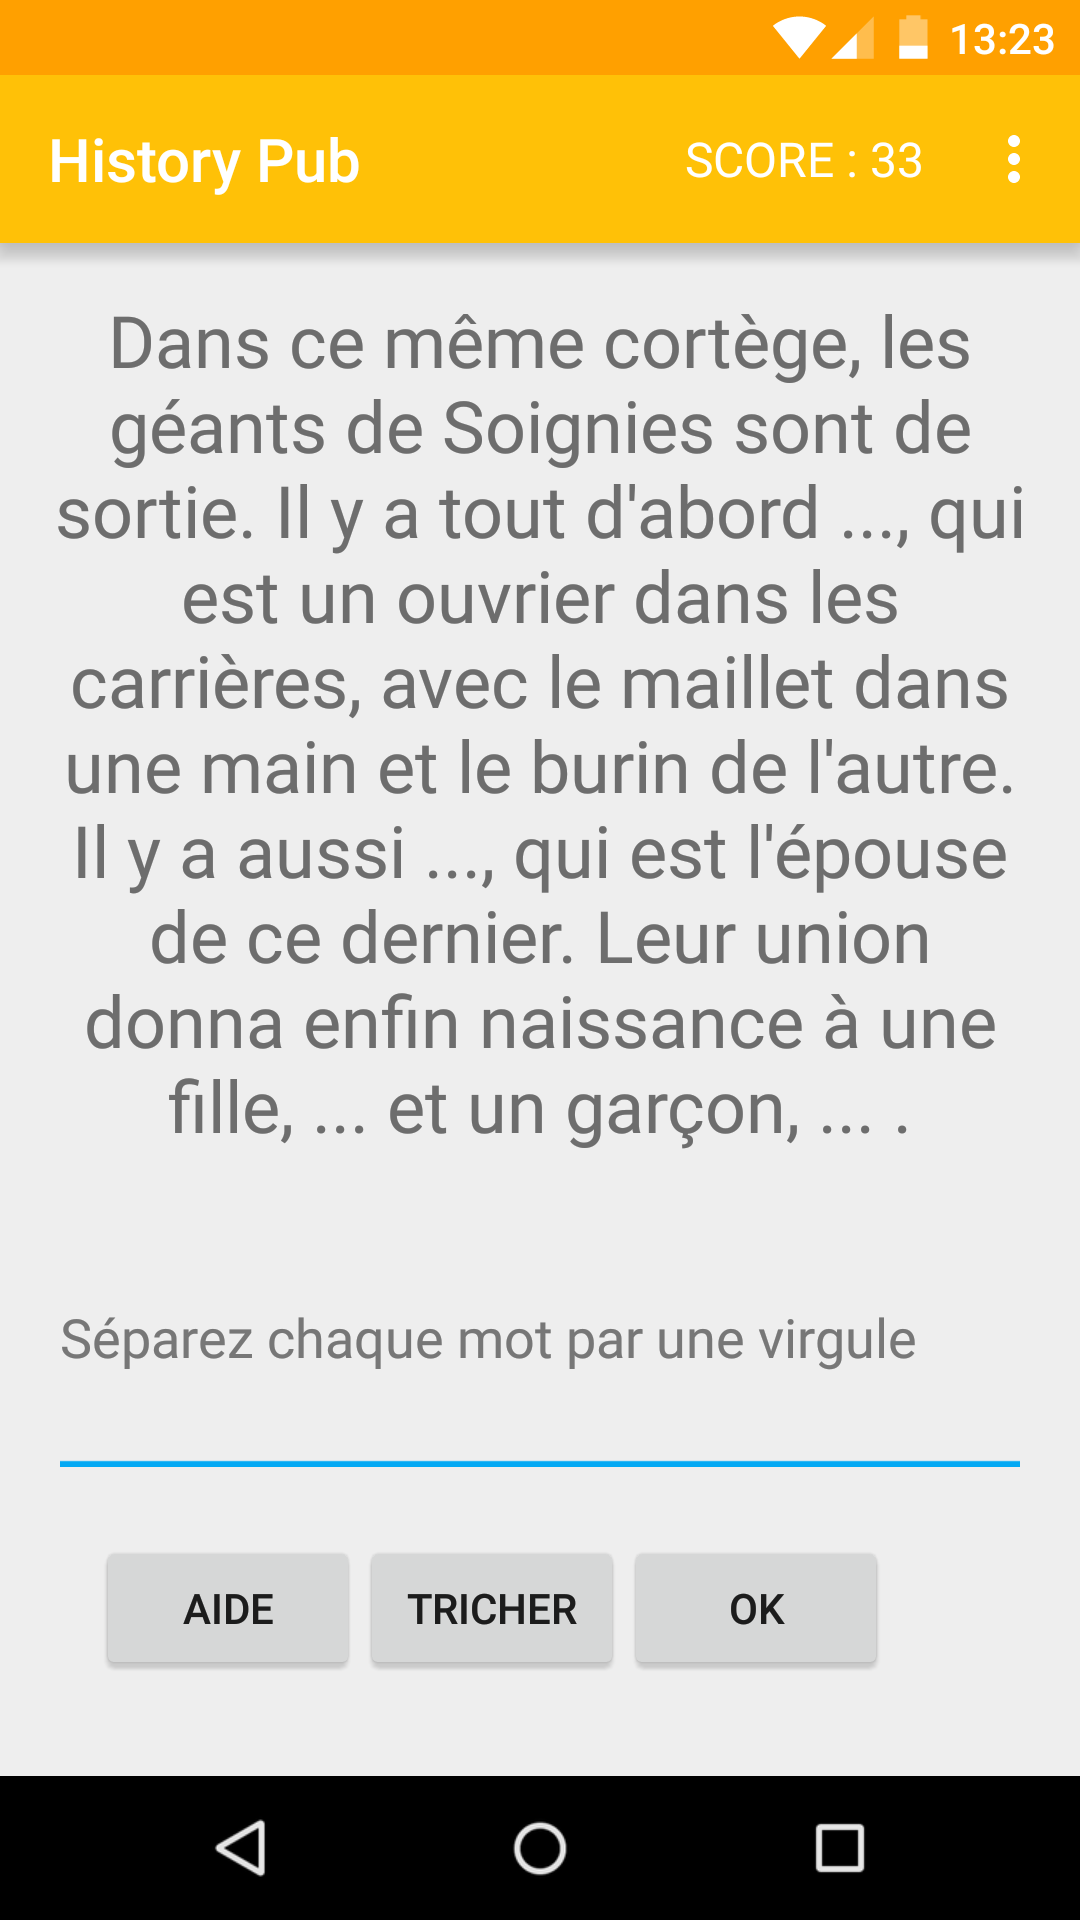
\includegraphics[scale=.25]{images/trou1.png}}\quad\quad\quad
        \subfigure{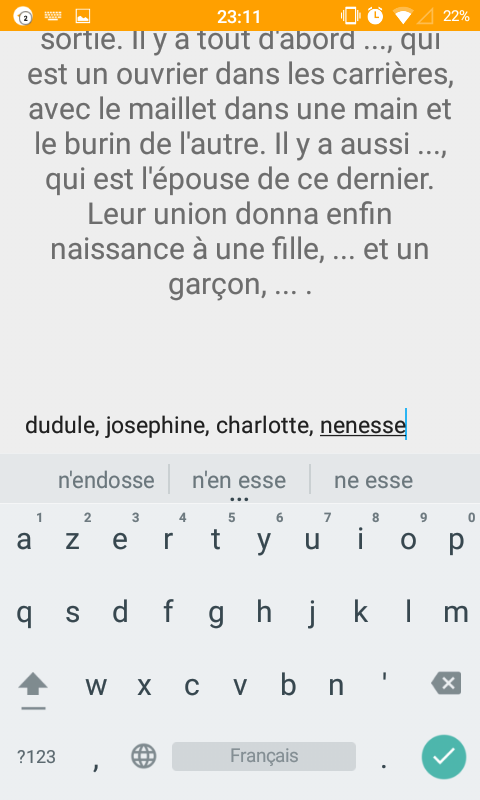
\includegraphics[scale=.25]{images/trou2.png}}}
        \caption{Question à trous, avant et après avoir entré une réponse}
    \end{figure}
    Pour réponse à une question de texte à trous, il vous suffit d'entrer les différents mots manquants dans l'unique champs de texte. Ces différents mots doivent être séparés par une virgule. Seules les réponses comprenant tous les mots corrects sont acceptées.

    Pour ce type d'épreuve:
    \begin{description}[style=nextline]
        \item[Bouton de triche]Il remplit automatiquement le champs de réponse avec la ou les bonne(s) réponse(s). Aucune modification ne sera alors possible dans cet EditText. Il faut ensuite appuyer sur le bouton OK.
        \item[Bouton d'aide]Il remplit automatiquement le champs de réponse avec la première lettre de chaque mot, et une virgule entre les différentes lettres ainsi révélées. Il faudra cependant compléter la réponse.
    \end{description}

    \section{Epreuve Question Ouverte}
    \begin{figure}[H]
        \centering
        \mbox{\subfigure{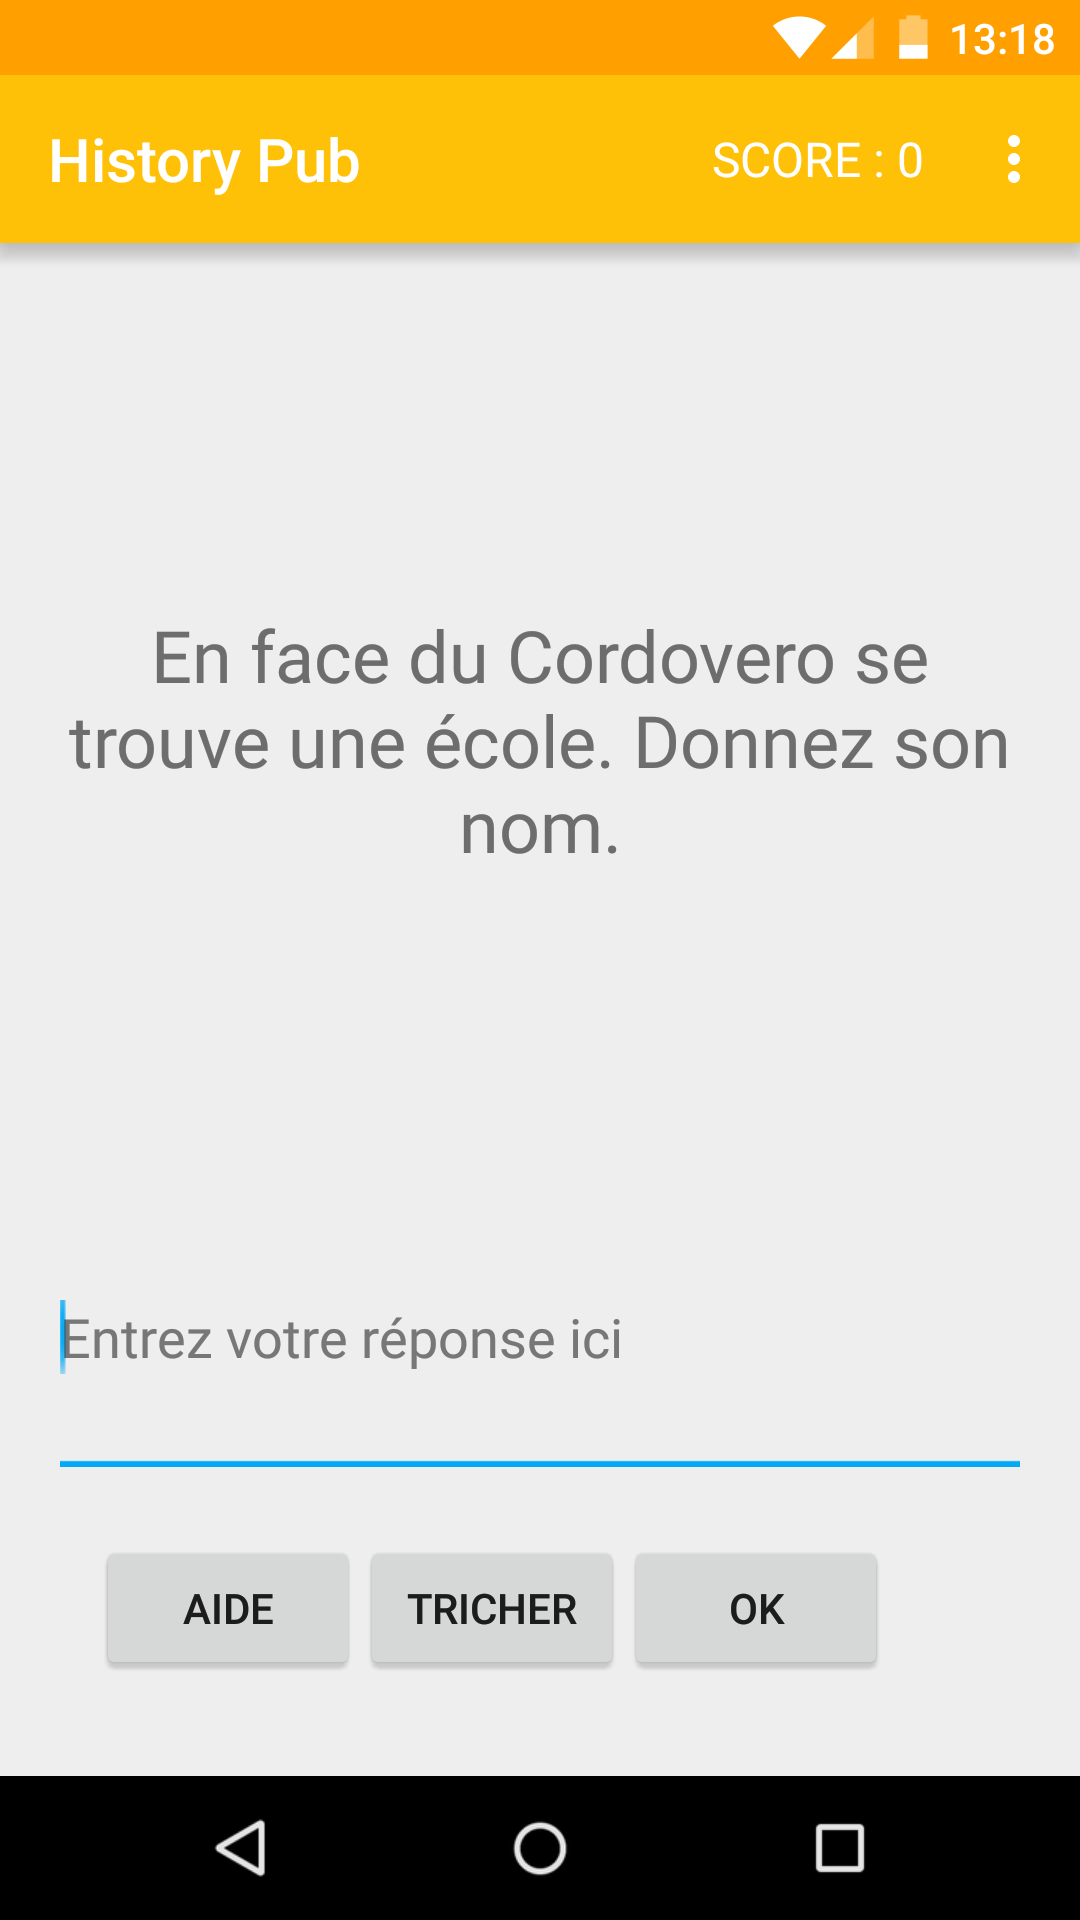
\includegraphics[scale=.25]{images/ouverte1.png}}\quad\quad\quad
        \subfigure{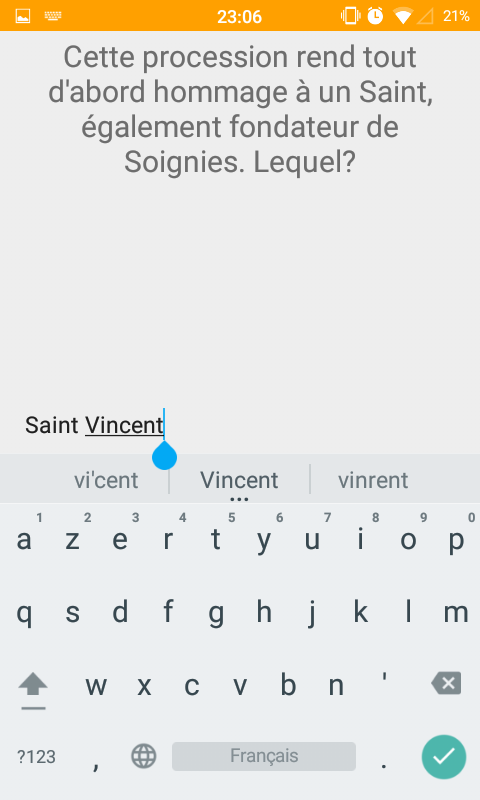
\includegraphics[scale=.25]{images/ouverte2.png}}}
        \caption{Question ouverte, avant et après avoir entré une réponse}
    \end{figure}
    Pour répondre à une question ouverte, il vous suffit de taper la réponse demandée. Cette réponse est unique mais peut être entrée de différente manière. Par exemple pour une question dont la réponse attendu serait \og Institut Paul Lambin\fg, la réponse \og IPL\fg serait aussi acceptée.\\

    Une fois la réponse entrée, vous pouvez confirmer votre solution avec la bouton entré de votre clavier virtual ou, après avoir quitté ce clavier, avec la bouton OK.

    Pour ce type d'épreuve:
        \begin{description}[style=nextline]
            \item[Bouton de triche]Il remplit automatiquement le champs de réponse avec la bonne réponse. Aucune modification ne sera alors possible dans cet EditText. Il faut ensuite appuyer sur le bouton OK.
            \item[Bouton d'aide]Il remplit automatiquement le champs de réponse avec la première lettre de la réponse. Il faudra cependant compléter la réponse.
        \end{description}

    \section{Epreuve Photographique}
    % mettre un screenshot

    Pour répondre à une question phorotgaphique, il vous suffit de vous trouver dans la zone requise et de prendre une photo du batiment ou autre objet demandé. Une fois la photo prise, vous avez un aperçu de l'image et il ne vous reste plus qu'à accepter cette photo.\\

    Aucune vérification n'est faite sur ce type d'épreuve. Faites donc de votre mieux, on compte sur vous!

    Pour ce type d'épreuve:
    \begin{description}[style=nextline]
        \item[Bouton de triche]Il affiche automatiquement la bonne image dans la zone de prévisualisation. Il faut ensuite appuyer sur le bouton OK.
        \item[Bouton d'aide]Il affiche automatiquement la bonne image dans la zone de prévisualisation pendant 5 secondes. Il faudra cependant prendre une photo.
    \end{description}

    \textit{Remarque: }Les épreuves photographiques ne sont pas géolocalisées, bien que cela le devrait.

    \section{Fin du jeu}
    \begin{figure}[H]
        \centering
        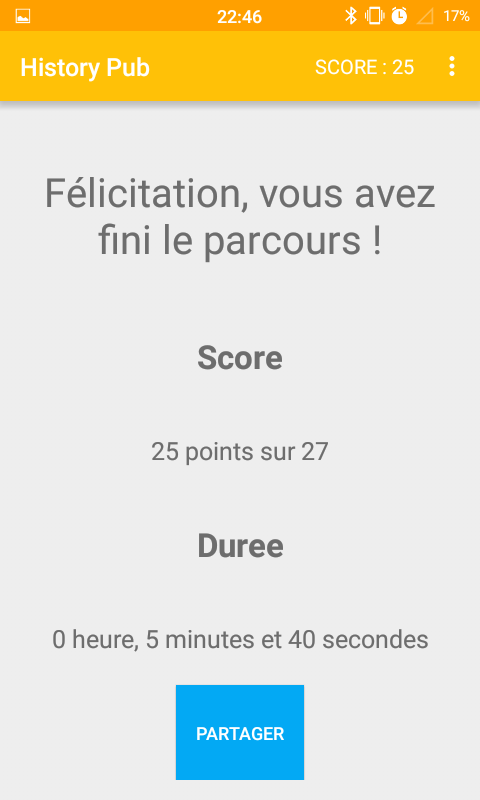
\includegraphics[scale=.25]{images/final.png}
        \caption{Ecran final}
    \end{figure}

    Une fois tout le parcours fini, vous serez face à un écran récapitulatif vous permettant de savoir le nombre de points que vous avez marqués ainsi que le temps que vous avez mis pour finir ce parcours.\\

    Cette page vous permet aussi de partager votre score avec vos connaissances ainsi que de les mettre au défi de vous battre!

    \section{Informations générales}
    \begin{figure}[H]
        \centering
        \mbox{\subfigure{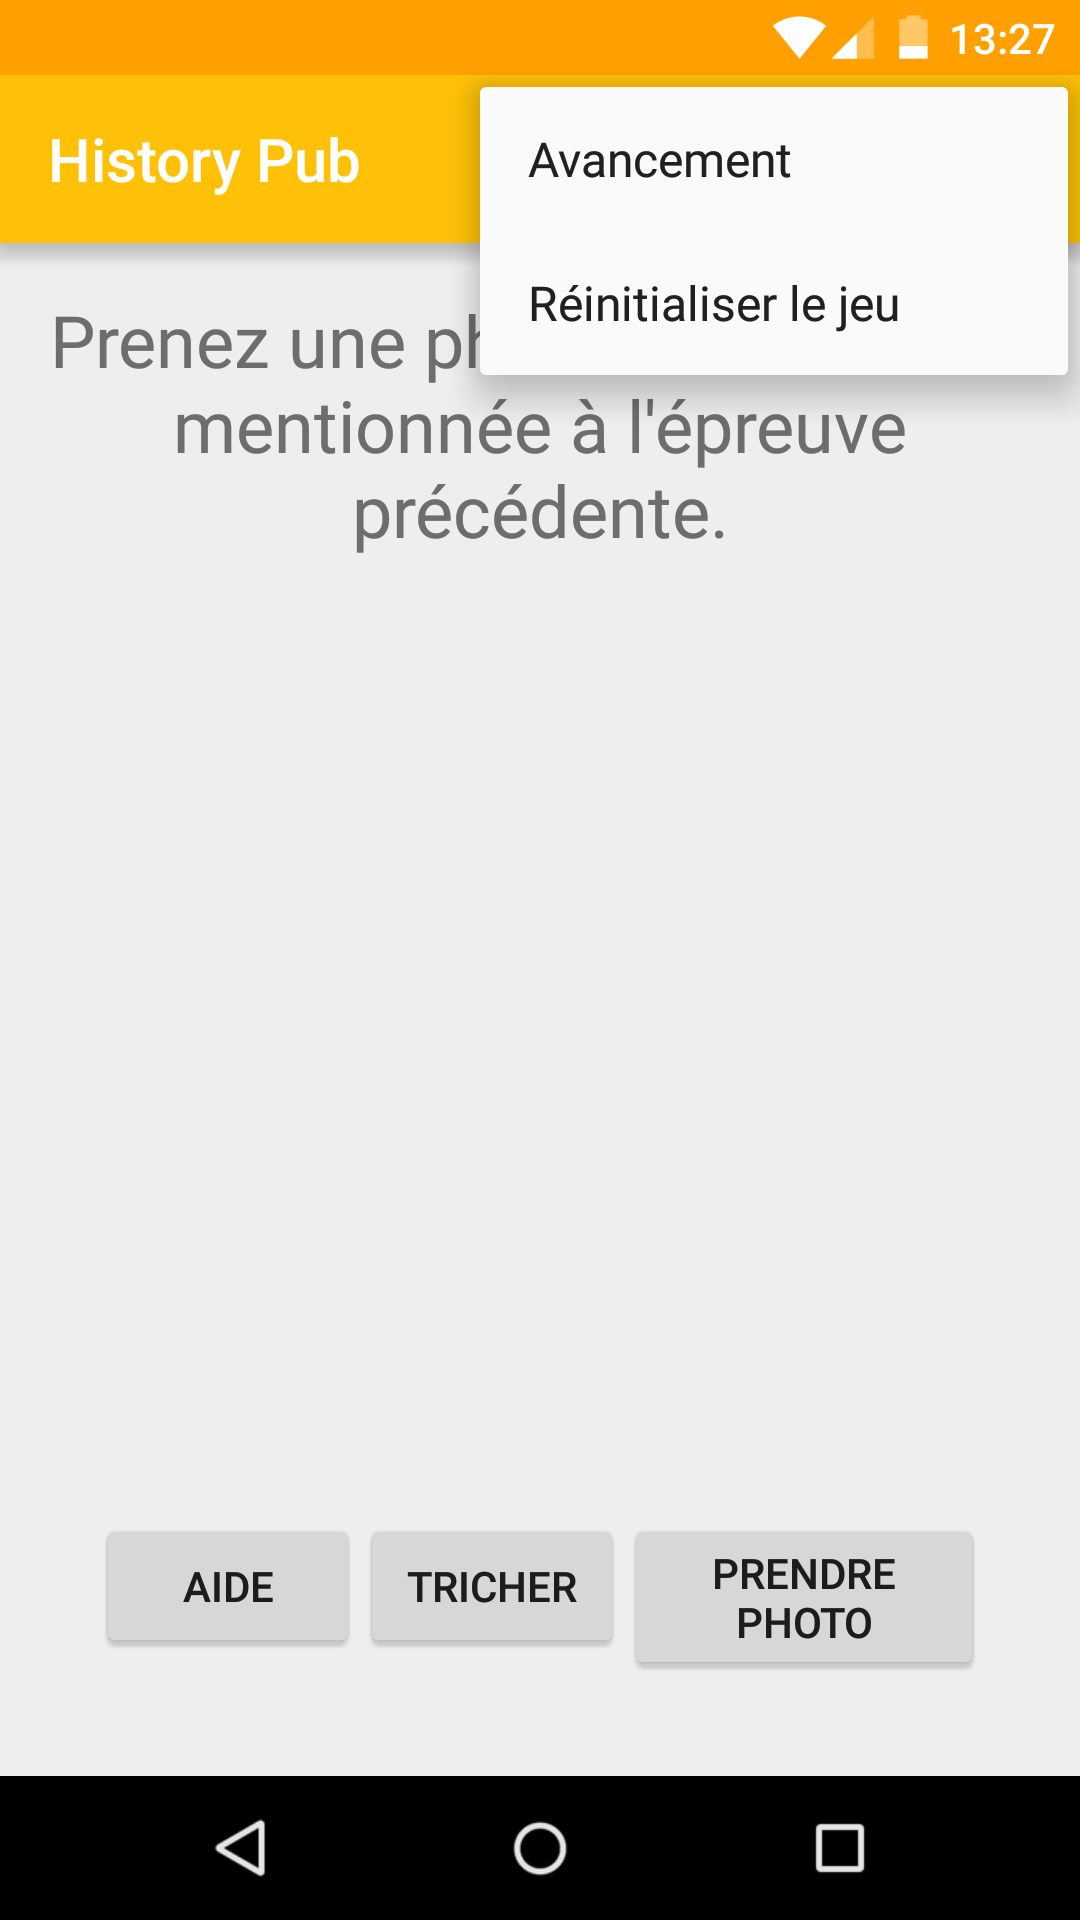
\includegraphics[scale=.25]{images/menu.png}}\quad\quad\quad
        \subfigure{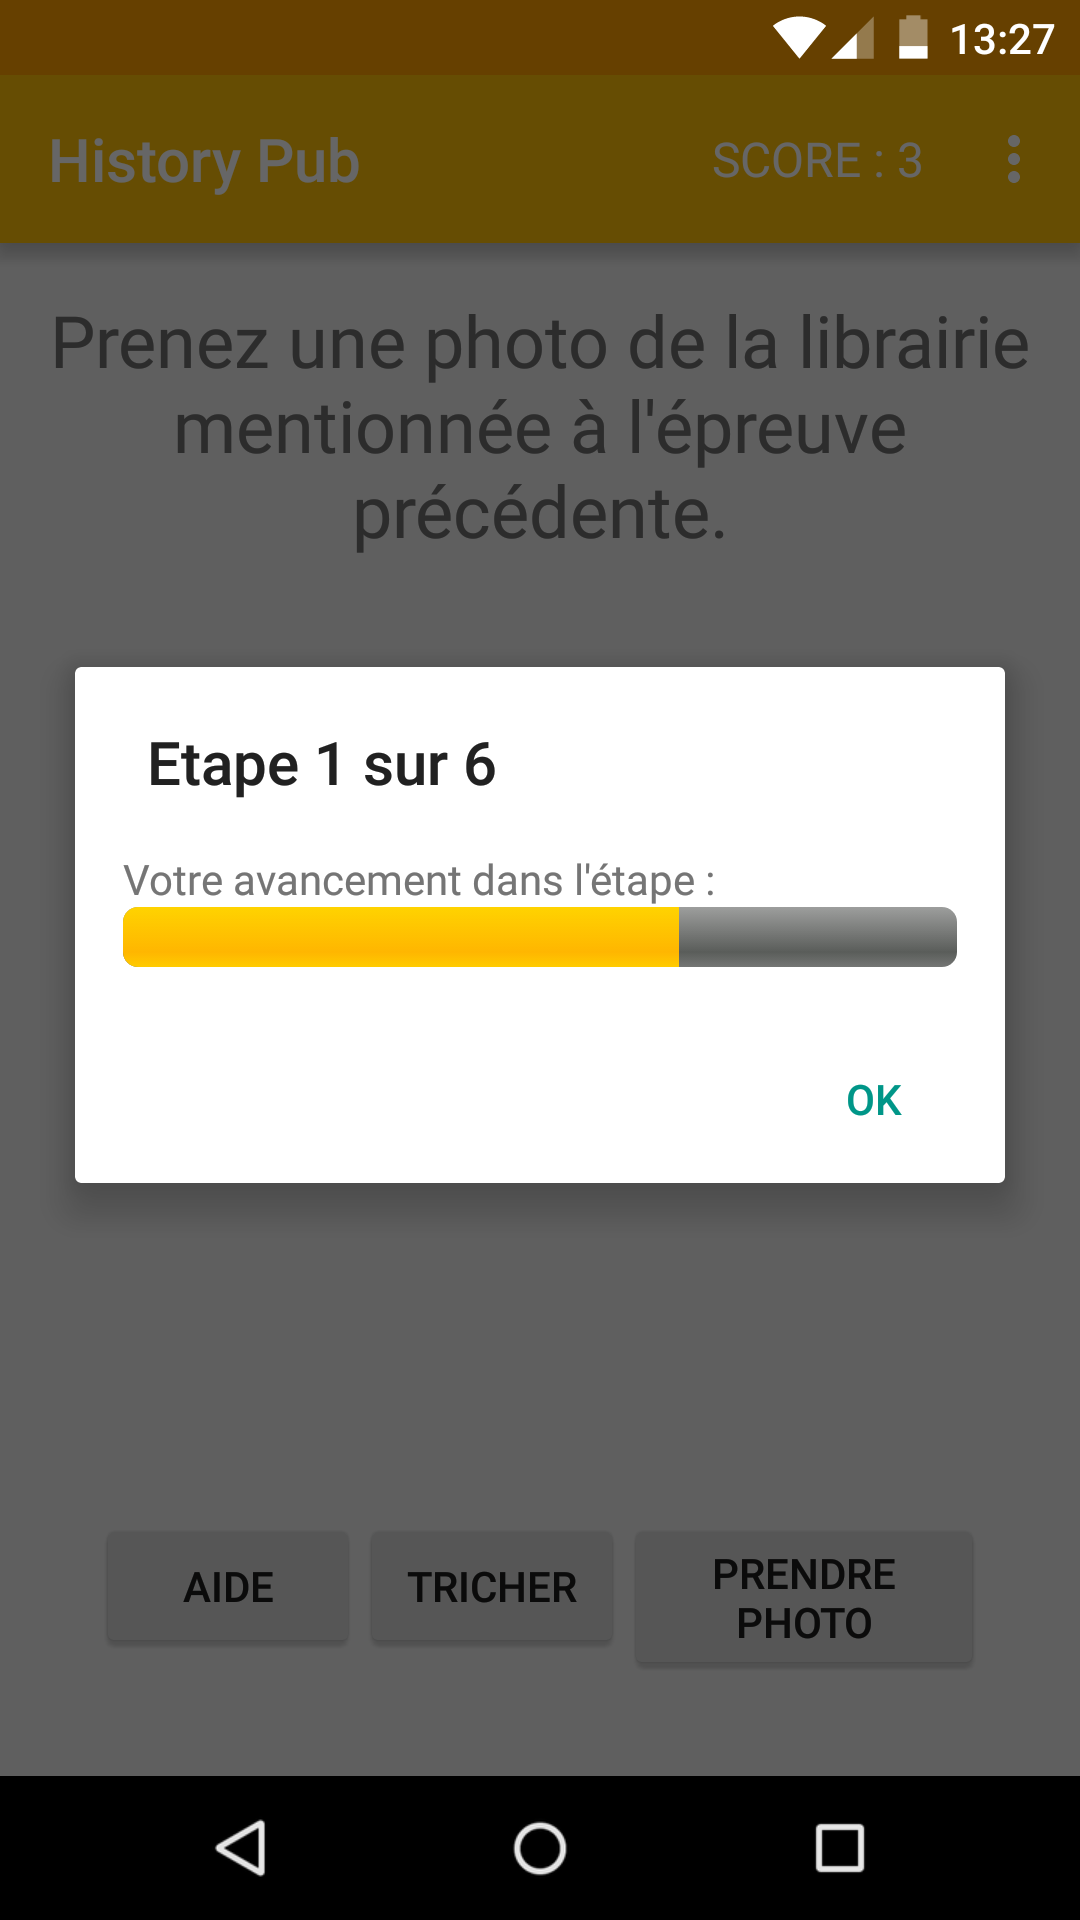
\includegraphics[scale=.25]{images/avancement.png}}}
        \caption{Menu de la barre d'action et popup d'avancement}
    \end{figure}

    A tout instant durant le jeu, vous avez la possibilité de voir votre score dans la barre d'action de vottre application.\\

    Vous pouvez aussi, via le menu de cette barre d'action, voir votre avancement ou remettre le jeu à zéro. Ces deux actions sont montrées dans les captures d'écran ci-dessus.

    \chapter{Architecture}
    L'architecture de l'application suit, autant que faire se peut, les règles énoncées par \textsc{Google}.\\

    Les messages et autres chaines de caractères affichés à l'utilisateur sont repris dans le fichier \textit{string.xml}, permettant une traduction et donc une localisation aisée. Certains éléments visuels ont un style et des caractéristiques communs repris dans le fichier \textit{styles.xml}, permettant de mettre à jour le design de l'application de façon simple et sans devoir rechercher dans les différents fichiers de layout.\\

    Concernant le code java, nous avons suivi les conventions de nommage des attributs énoncés par l' \textsc{Android Open Source.Project}. C'est à dire que :
    \begin{itemize}
        \item les attributs \textbf{non public}, \textbf{non static} commencent par un m
        \item les attributs \textbf{static} commencent par un s
        \item les autres attributs commencent par une lettre minuscule
        \item les attributs \textbf{public static final} s'écrivent en MAJUSCULE\_AVEC\_UNDERSCORES
    \end{itemize}

    Le code est de plus, bien entendu, commenté et contient de la javadoc la plus compréhensible possible.\\

    Concernant les classes java, nous avons séparé les classes dite \og POJO\fg, qui sont de simples objets Java de classes relative à \textsc{Android}, c'est à dire les activités ainsi que des \og User Case Controller\fg{} (Correspondant ici à la classe gérant le fichier XML et également le déroulement du jeu).

    Dans les POJO, nous avons différentes classes, correspondant aux différentes épreuves, aux étapes ainsi qu'à une zone autour d'un point géographique.

    Les activités elles correspondent chacune à une étape, épreuve ou autre écran affiché à l'utilisateur. Elles gèrent donc l'interaction entre l'utilisateur et l'interface visuelle. L'interface en elle-même étant gérées par les fichier XML du dossier layout.

    L'UCC gère le chargement du fichier XML et est implémenté en tant que \textbf{singleton}. Celà permet de charger le jeu complet en une seule fois (comprenez les différentes étapes, épreuves et tout ce qui les compose) et de permettre par la suite à toutes les activités de piocher l'étape et/ou l'épreuve qui lui est nécessaire.

    Nous avons bien conscience que le pattern Singleton n'est plus vu comme une bonne pratique voire même comme un anti-pattern, mais n'ayant aucune connaissance en injection de dépendance sur la plateforme d'Android, nous avons finalement opté pour ce pattern.

    \chapter{Bugs connus}
    Le seul bug connu à ce jour réside dans l'affichage des questions & propositions de réponses sur les petits écrans. En effet, ceux-ci sont hachés (entendez par là que le texte dépasse de l'emplacement prévu) et il est donc impossible de les lire dans leur entièreté.
    Nous avons cependant plusieurs pistes pour le résoudre:
     \begin{itemize}
         \item Ajout d'un ScrollView pour les questions. Dans ce cas, les questions nécessitant trop de place seront lisibles en scrollant.
         \item Créer un dossier values pour petits écrans. Dans ce cas, les styles (donc la taille de la police, des layouts, ...) seraient adaptés en fonction de la taille de l'écran.
         \item Combinaison des 2 solutions ci-dessus.
     \end{itemize}
     Dans notre cas, nous avions opté pour la solution n°2 (la solution n°1 ne nous convenait pas et la solution n°3 était trop ambitieuse dans le temps imparti). Cependant, par manque de temps, nous n'avonc pas réussi à mettre cette solution en place.

    \chapter{Utilisation de code open-source}
    Le code de \textsc{History Pub} reprend, à certains endroits précis, du code open-source. Ces parties de code open-source se retrouvent ci-dessous :

    \begin{description}[style=nextline]
        \item[EtapeActivity.java et PhotoActivity.java] La partie géolocalisation reprends en grande partie du code fournis par \textsc{Google} sur leur plateforme \url{developer.android.com} ainsi que sur \textsc{Github} à cette adresse: \url{https://github.com/googlesamples/android-play-location}. Ce code est fourni sous la license \textbf{Apache}, permettant son inclusion dans un projet sous license \textbf{GPLv3}.
        \item[PhotoActivity.java] La partie prise de photo reprends le code fournis par \textsc{Google} sur la plateforme précédemment citée, toujours sous la license \textbf{Apache}.
        \item[PhotoActivity.java] La méthode permettant de charger et d'afficher une image depuis les assets (lors d'un cheat ou d'une aide), provient de \textsc{StakOverflow} à cette adresse : \url{http://stackoverflow.com/a/11734899}. Le code se trouvant sur \textsc{StackOverflow} est sous licence \textbf{Apache}, qui est donc compatible avec la \textbf{GPLv3}.
        \item[Style.css] Le design des boutons, façon Material Design, est repris du \textsc{Codepen} créé par RayCh et trouvable à cette adresse : \url{http://codepen.io/iraycd/pen/dHrxv}. Le code posté sur \textsc{Codepen} est sous license \textbf{MIT}, elle aussi compatible avec la \textbf{GPLv3}.
    \end{description}

    \chapter{License}

    \noindent \textsc{History Pub} est placé sous license GNU GENERAL PUBLIC LICENSE version 3.
    \hfill\\

    \noindent Cela signifie que n'importe qui \textbf{peut} :
    \begin{itemize}
        \item utiliser notre code de façon privée
        \item utiliser notre code dans des projets à but commercial
        \item redistribuer notre code
        \item modifier notre code
    \end{itemize}
    \hfill\\
    Mais cela signifie aussi qu'une personne utilisant tout ou partie du code de \textsc{History Pub} dans un projet \textbf{doit} :
    \begin{itemize}
        \item publier les sources de ce projet
        \item inclure une copy de la license et copyright dans ce projet
        \item préciser les changements importants fait à notre code
    \end{itemize}
    \hfill\\
    Celà signifie aussi que notre code est fourni sans garantie et que nous ne pouvons donc pas être tenus responsable de problèmes quelconques liés à son utilisation en dehors de \textsc{History Pub}.
    \hfill\\

    \noindent Pour plus d'information, la license complète peut être trouvée à l'adresse suivante : \url{https://www.gnu.org/licenses/gpl.html}\\

    Le code source de l'application peut quant à lui être trouvé sur \textsc{Github} à l'adresse suivant : \url{https://github.com/Crapoo/HistoryPub}. Le code remis avec ce rapport correspond au commit \textsc{hash du commit}.

\end{document}
